%%% 吸收填料塔优化
\chapter{吸收填料塔成本、安全优化}

现考虑吸收填料塔设计的优化,因吸收塔内部、外部附件的选择取决于吸收塔工艺参数,当吸收填料塔任务目标及外界条件确定时,则整个填料塔对象各项参数确定。也就是说,选定的气体的流量、气体中\ce{SO2}的摩尔分数、\ce{SO2}的吸收率、操作温度、操作压力、填料总比表面积、填料直径、单个填料吸收塔高度限制、实际液气比取最小液气比的比率一定时,填料塔的工艺参数即可确定,所需成本价格、安全因素即确定。



%%% ===============================================
\section{变量分析}

\subsection{变量趋势分析}

为了更直观地了解各个变量对成本因素和安全因素的影响,我们绘制了变量趋势图。图\ref{fig:trends}展示了9个变量(即对象初始化的9个决策变量)分别对成本因素和安全因素的影响趋势。

\begin{figure}[hbtp]
	\centering
	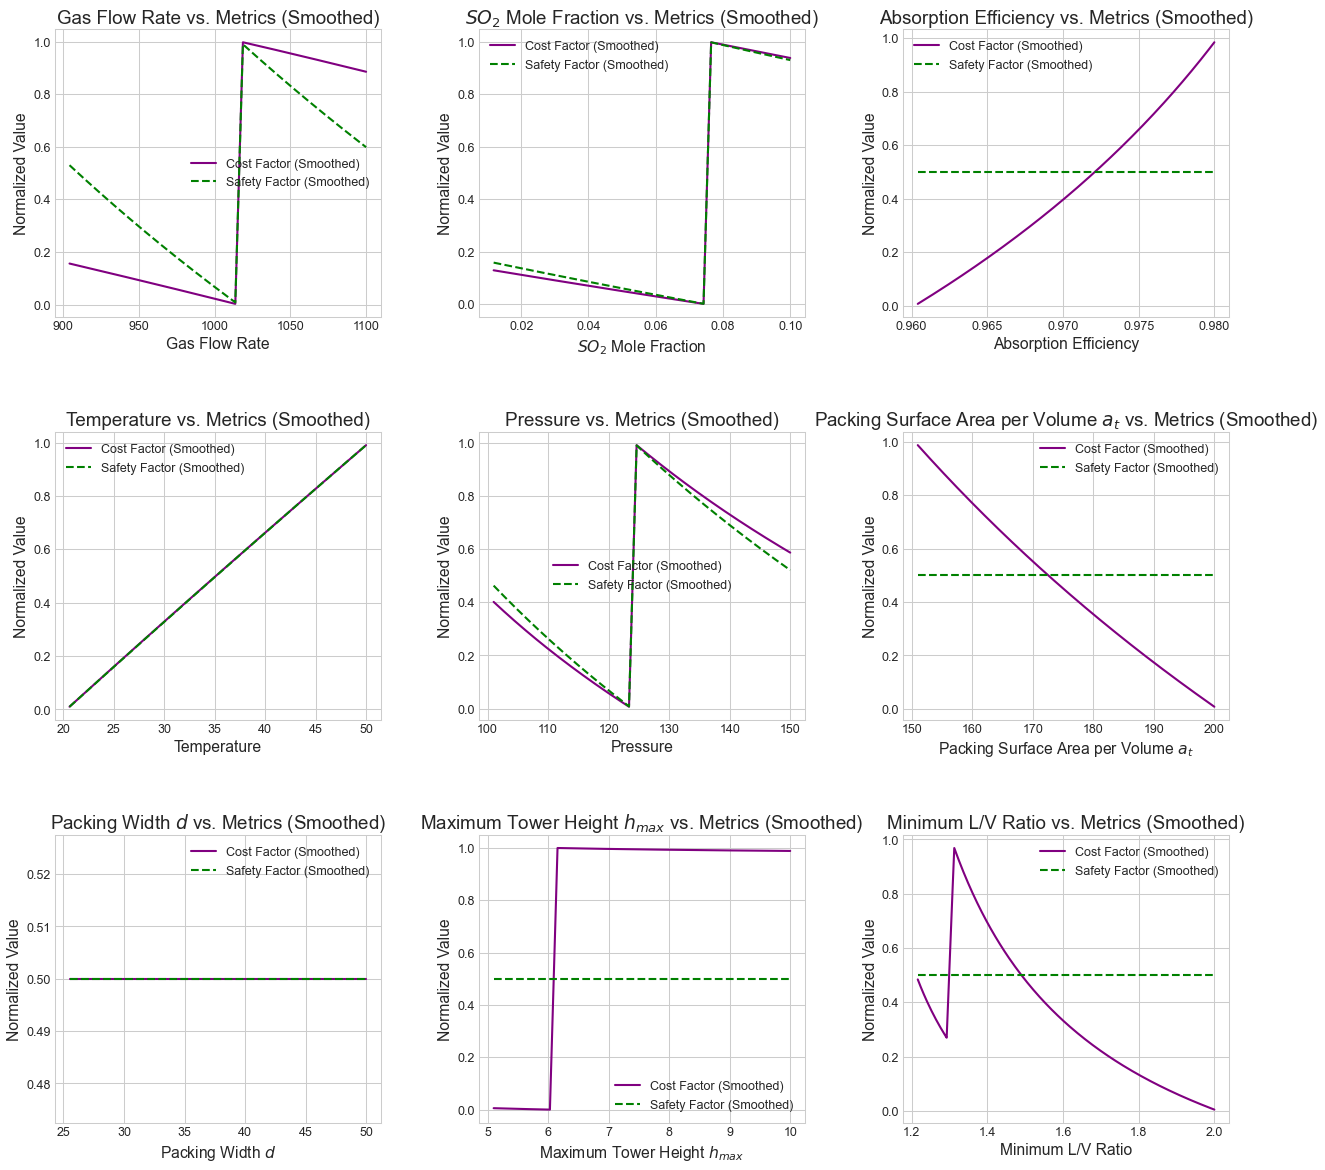
\includegraphics[width=0.8\textwidth]{trends.png}
	\caption{决策变量对成本因素和安全因素的影响趋势}
	\label{fig:trends}
\end{figure}

\clearpage

从图中可以观察到:

\begin{itemize}
	\item 气体流量的增加会导致成本因素和安全因素同时上升。
	\item 气相中二氧化硫含量的增加会导致成本因素下降,但安全因素也会降低。
	\item 二氧化硫吸收率的提高会增加成本因素,但同时也会提高安全因素。
\end{itemize}

这些趋势分析为我们后续的多目标优化提供了重要的参考。

\subsection{相关性分析方法}

为了确定哪些变量对成本因素和安全因素影响最大,我们进行了相关性分析。具体步骤如下:

\begin{enumerate}
	\item 对每个变量,在其可能的取值范围内取200个均匀分布的点。
	\item 固定其他变量,仅改变当前变量的值。
	\item 计算每个点对应的成本因素和安全因素。
	\item 使用Pearson相关系数计算变量与成本因素、安全因素的相关性。
\end{enumerate}

相关性系数的计算公式如下:

\begin{equation}
	r = \frac{\sum_{i=1}^{n} (x_i - \bar{x})(y_i - \bar{y})}{\sqrt{\sum_{i=1}^{n} (x_i - \bar{x})^2} \sqrt{\sum_{i=1}^{n} (y_i - \bar{y})^2}}
\end{equation}
其中,$x_i$和$y_i$分别表示变量和因素(成本或安全)的值,$\bar{x}$和$\bar{y}$表示它们的平均值。

\subsection{相关性分析结果}

通过相关性分析,我们得到了每个变量与成本因素和安全因素的相关系数。结果如表\ref{tab:correlation}所示。

\begin{table}[h]
	\centering
	\caption{变量与成本因素和安全因素的相关系数}
	\label{tab:correlation}
	\begin{tabular}{lcc}
		\hline
		变量 & 成本因素相关性 & 安全因素相关性 \\
		\hline
		气体流量 & 0.8036 & 0.5080 \\
		气相中二氧化硫含量 & 0.7276 & 0.7137 \\
		二氧化硫吸收率 & 0.9951 & -0.0000 \\
		操作温度 & 1.0000 & 1.0000 \\
		操作压力 & 0.6063 & 0.5222 \\
		填料总比表面积 & -0.9981 & 0.0000 \\
		填料直径 & nan & -0.0000 \\
		单个填料吸收塔最大高度 & -0.7055 & 0.0000 \\
		取最小液气比的比例常数 & -0.6191 & -0.0000 \\
		\hline
	\end{tabular}
\end{table}

根据相关性分析结果,可选择相关性最高的几个变量作为关键变量进行后续优化。

\section{多目标优化}

\subsection{基本假设}

\begin{enumerate}
	\item 吸收填料塔的成本因素仅与塔径和塔高有关。
	\item 填料的成本与填料塔的体积成正比。
	\item 不考虑塔内附件和塔外附件对成本、安全的影响,因填料塔工艺参数及填料确定内外附属部件可由此确定,所需成本也随即确定。
\end{enumerate}

\subsection{决策变量}
现对如下九个变量关于成本因素、安全因素进行相关性分析和趋势性分析。

\begin{enumerate}
	\item 气体流量,$V$
	\item 气相中二氧化硫含量,$Y_{1}$
	\item 二氧化硫吸收率,$\eta$
	\item 操作温度,$T$
	\item 操作压力,$P$
	\item 填料总比表面积,$a_{t}$
	\item 填料直径,$d$
	\item 单个填料吸收塔最大高度,$h_{max}$
	\item 取最小液气比的比例常数,$\big(\frac{L}{V}\big)_{min\,ratio}$
\end{enumerate}

\subsection{优化目标}

本章节优化目标为:
\begin{enumerate}
	\item 最小化吸收填料塔的成本因素,$Cost\,Factor$
	\item 最大化吸收填料塔的安全因素,$Safety\,Factor$
\end{enumerate}

这两个目标通常是相互矛盾的,因为提高安全性通常会增加成本。因此,我们需要在这两个目标之间寻找一个平衡点。

基于前面的分析,我们将吸收填料塔的优化问题定义为一个多目标优化问题:

\begin{equation}
	\begin{aligned}
		& \text{minimize}   & & f_1(\mathbf{x}) \quad \text{(成本因素)} \\
		& \text{maximize}   & & f_2(\mathbf{x}) \quad \text{(安全因素)} \\
		& \text{subject to} & & \mathbf{x}_l \leq \mathbf{x} \leq \mathbf{x}_u
	\end{aligned}
\end{equation}
其中,$\mathbf{x}$是决策变量向量,$\mathbf{x}_l$和$\mathbf{x}_u$分别是决策变量的下界和上界。

\subsection{NSGA-II算法}

为了解决这个多目标优化问题,我们选择使用NSGA-II(Non-dominated Sorting Genetic Algorithm II)算法。NSGA-II是一种高效的多目标优化算法,它具有以下特点:

\begin{itemize}
	\item 使用快速非支配排序方法
	\item 采用拥挤度距离来保持解的多样性
	\item 精英策略,确保最优解不会在进化过程中丢失
\end{itemize}

NSGA-II的主要步骤如下:

\begin{enumerate}
	\item 初始化种群
	\item 对种群进行非支配排序
	\item 计算拥挤度距离
	\item 选择、交叉和变异操作生成子代
	\item 合并父代和子代,进行精英选择
	\item 重复步骤2-5,直到达到终止条件
\end{enumerate}

\subsection{优化结果}

通过运行NSGA-II算法,我们得到了一系列非支配解,即帕累托前沿。图\ref{fig:pareto}展示了优化结果的帕累托前沿。

\begin{figure}[h]
	\centering
	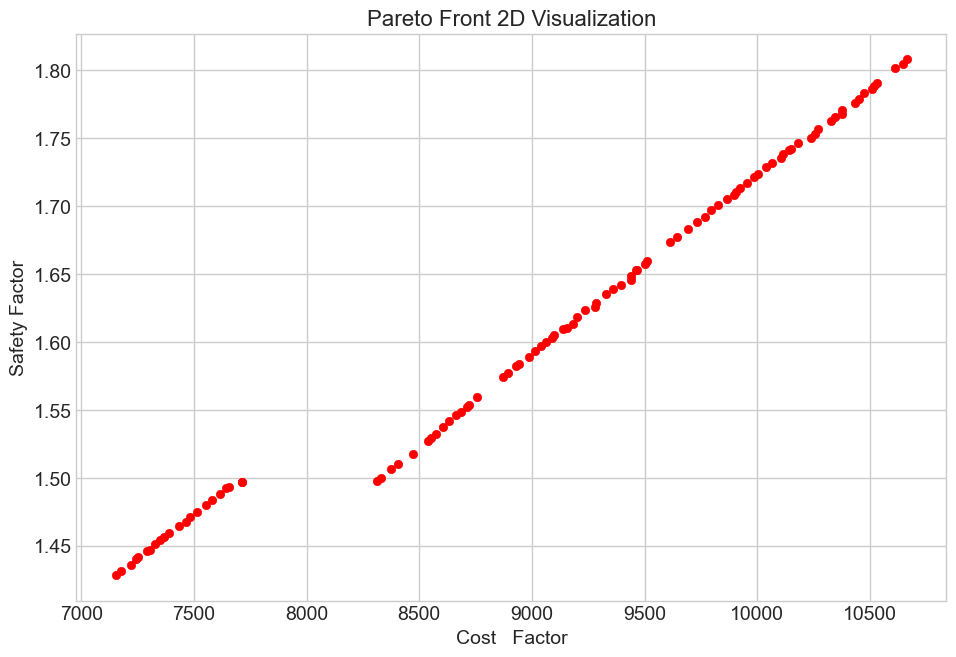
\includegraphics[width=\textwidth]{pareto_front.png}
	\caption{优化结果的帕累托前沿}
	\label{fig:pareto}
\end{figure}

从帕累托前沿可以看出,成本因素和安全因素之间存在明显的权衡关系。决策者可以根据具体需求,从帕累托前沿上选择合适的解。

表\ref{tab:optimal_solutions}列出了帕累托前沿上的一些代表性解。

\begin{table}[h]
	\footnotesize
	\centering
	\caption{帕累托前沿上的代表性解}
	\label{tab:optimal_solutions}
	\begin{tabular}{cccccccccc}
		\hline
		解 & 气体流量 & \ce{SO2}含量 & 吸收率 & 温度 & 压力 & 填料比表面积 & 填料宽度 & 最大塔高 & 最小$\big(\frac{L}{V}\big)$比率 \\
		\hline
		1 & 49.77 & 300.00 & 0.96 & 900.05 & 0.01 & 109.72 & 42.91 & 9.68 & 2.00 \\
		2 & 49.73 & 295.97 & 0.96 & 900.03 & 0.01 & 109.72 & 42.77 & 9.79 & 2.00 \\
		3 & 49.79 & 300.00 & 0.96 & 900.00 & 0.07 & 149.89 & 41.70 & 9.79 & 2.00 \\
		4 & 50.00 & 300.00 & 0.96 & 900.03 & 0.01 & 100.03 & 42.58 & 9.97 & 2.00 \\
		5 & 49.77 & 300.00 & 0.96 & 900.08 & 0.02 & 143.88 & 43.84 & 10.00 & 2.00 \\
		6 & 49.70 & 300.00 & 0.96 & 900.00 & 0.02 & 118.19 & 39.48 & 9.99 & 2.00 \\
		7 & 49.99 & 299.99 & 0.96 & 900.02 & 0.01 & 143.49 & 34.46 & 9.69 & 2.00 \\
		8 & 49.97 & 299.97 & 0.96 & 900.01 & 0.03 & 118.54 & 33.68 & 8.79 & 2.00 \\
		9 & 49.97 & 299.97 & 0.96 & 900.01 & 0.01 & 111.59 & 33.69 & 8.77 & 2.00 \\
		10 & 49.99 & 300.00 & 0.96 & 900.02 & 0.01 & 114.97 & 34.44 & 9.51 & 2.00 \\
		\hline
	\end{tabular}
\end{table}

\clearpage

\begin{table}[h]
	\small
	\centering
	\caption{优化结果的代表性目标值}
	\label{tab:objective_values}
	\begin{tabular}{c@{\hspace{0.35\textwidth}}r@{\hspace{0.3\textwidth}}c}
		\hline
		优化结果 & 成本因素 & 安全因素 \\
		\hline
		1 & 7107 & 1.43 \\
		2 & 10658 & 1.81 \\
		3 & 8255 & 1.50 \\
		4 & 7627 & 1.50 \\
		5 & 8786 & 1.57 \\
		6 & 10001 & 1.73 \\
		7 & 8851 & 1.58 \\
		8 & 9911 & 1.72 \\
		9 & 10459 & 1.79 \\
		10 & 10250 & 1.76 \\
		\hline
	\end{tabular}
\end{table}

通过对吸收填料塔的多目标优化研究,我们得出以下结论:

\begin{enumerate}
	\item 气体流量、\ce{SO2}含量和吸收率是影响成本因素和安全因素最显著的变量。
	\item 成本因素和安全因素之间存在明显的权衡关系,无法同时实现两者的最优。
	\item NSGA-II算法能够有效地找到吸收填料塔设计的帕累托最优解集。
\end{enumerate}

基于以上结论,我们提出以下建议:

\begin{enumerate}
	\item 在实际设计中,应根据具体需求在成本和安全之间寻找平衡点。
	\item 可以考虑使用本研究中的优化方法来辅助吸收填料塔的设计决策。
	\item 在条件允许的情况下,可以进一步考虑其他因素(如环境影响)进行多目标优化。
\end{enumerate}